%% En-tête
\documentclass[a4paper,12pt,titlepage]{article}
\usepackage[french]{babel}
\usepackage[utf8]{inputenc} % encodage
\usepackage[T1]{fontenc} % encodage
\usepackage{array} % tableaux
\usepackage[bookmarks=true,colorlinks,linkcolor=blue]{hyperref} % hyperliens
\usepackage{aeguill} % lisibilité
\usepackage{graphicx} % pour insérer des images
\usepackage{amssymb,amsmath} % maths
\usepackage{multicol} % colonnes
\usepackage[francais]{varioref} % chouettes refs
\usepackage{listingsutf8} % to allow utf8 with lstlisting
\usepackage{amsthm} % math proof
\usepackage{float} % mettre les figures où on veut

\lstset{
    language=C++,
    tabsize=3,
    showstringspaces=false, %pour virer les espaces dans les chaines de caractères
    %basicstyle=\ttfamily\footnotesize,
    %commentstyle=\color{Green}\scriptsize, % white comments
    %keywordstyle=\bfseries,
    %keywordstyle=\color{Blue}\textnormal,
    keywordstyle=\bfseries\ttfamily\color[rgb]{0,0,1},
    identifierstyle=\ttfamily,
    commentstyle=\color[rgb]{0.133,0.545,0.133},
    stringstyle=\ttfamily\color[rgb]{0.627,0.126,0.941},
    showstringspaces=false,
    basicstyle=\small,
    numberstyle=\footnotesize,
    title=\lstname, %afficher le titre
    frame=leftline, % le cadre
    captionpos=b, %légende en dessous
    numbers=left, %pour rajouter des numéros de ligne
    stepnumber=5, %définition du pas pour les numéros
    firstnumber=1, %définition du 1er numéro
    breaklines=true,      %pour casser les lignes trop longues
    caption=\lstname,
    inputencoding=utf8/latin1
}


%% Propriétés du document
\title{Compte-rendu de projet IF23\\Système autonome de manipulation de données GPS}
\author{Youenn Piolet \and Julien Nozais \and Alexandre Horréard}
\date{\today} % préférer la date réelle du TP


\begin{document}

\maketitle

\tableofcontents

\newpage

\section{Présentation du projet}

\subsection{Le travail réalisé}

Le but du projet est de créer un programme tournant sur un microcontrôleur
Arduino permettant de manipuler de gérer le fonctionnement d'un GPS, avec
affichage, sauvegarde et synchronisation via USB.

Notre boitier récupère les informations envoyées par le module GPS et les
stocke sur une carte SD dans des fichiers séparés. Ces fichiers peuvent
ensuite être récupérés sur un PC pour être utilisés avec GPSprune, un
logiciel permettant d'afficher le parcours correspondant aux données envoyées.

\bigskip
Un premier bouton permet de démarrer ou d'arrêter le parcours. Chaque nouveau
redémarrage créé un nouveau fichier d'enregistrement. Chaque parcours
est donc enregistré dans un fichier séparé. On peut également mettre
l'enregistrement sur pause et le redémarrer ensuite, sans changer de parcours.
(Utile pendant les pauses, ou un déplacement en voiture, en train, ne souhaitant
pas être enregistré).
\\
Le boitier dispose d'un écran LCD qui permet d'afficher plusieurs informations.
En appuyant sur un deuxième bouton on change l'affichage. L'écran peut afficher
les coordonnées, la vitesse, la distance parcourue ou l'heure. Toutes ces
informations sont mises à jour à chaque nouvelle réception de trame.
\\
Un autre bouton permet de choisir le mode d'enregistrement : soit les points
sont enregistrés suivant un temps fixe (toutes les trois secondes), soit ils le
sont suivant leur distance avec le point précédent. Nous obtenons ainsi une
suite de points qui ne sont pas identiques.
\\
L'ensemble fonctionne sur pile. Au démarrage du boitier, la batterie s'affiche
sur l'écran LCD.

\subsection{Mathématiques appliquées}

Pour calculer la distance entre deux points, on utilise la formule de Vincenty.
Il s'agit d'une méthode itérative pour calculer la distance entre deux points à
la surface d'un sphéroïde. Cette formule utilise l'hypothèse que la Terre est un
sphéroïde aplati aux pôles, ce qui les rend plus précise que d’autres méthodes
qui considèrent la terre comme parfaitement sphérique.

\subsection{Contraintes}

Nous avons atteint les limites de la mémoire de l'Arduino. Il a donc fallu
réduire au maximum l'empreinte mémorielle de notre programme. Notre code
étant entièrement orienté objet, nous avons malheureusement dû supprimer un
certain nombre de classes superflues. La classe String que nous utilisions
également étant trop lourde, nous avons pris la décision de la remplacer par
des tableaux de caractères, moins coûteux au prix d'un certain nombre de
fonctionnalités en moins.


\section{UML}

\subsection{Diagramme de cas d'utilisation}

\begin{figure}[H]
    \centering
    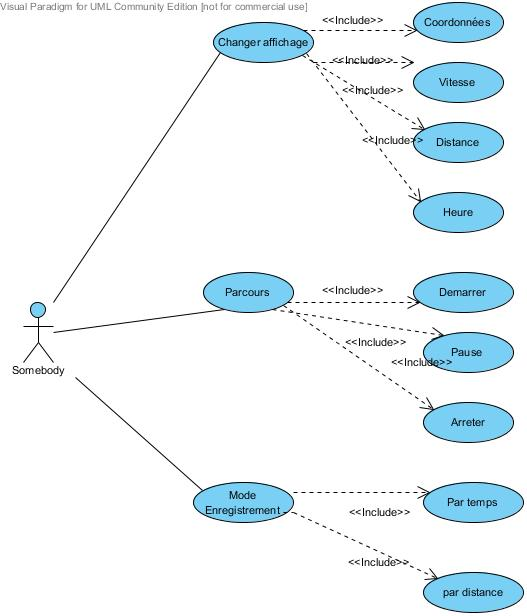
\includegraphics[width=\textwidth]{use_case.jpg}
    \caption{Diagramme de cas d'utilisations}
    \label{usecase}
\end{figure}

\subsection{Diagramme de séquence}

\begin{figure}[H]
    \centering
    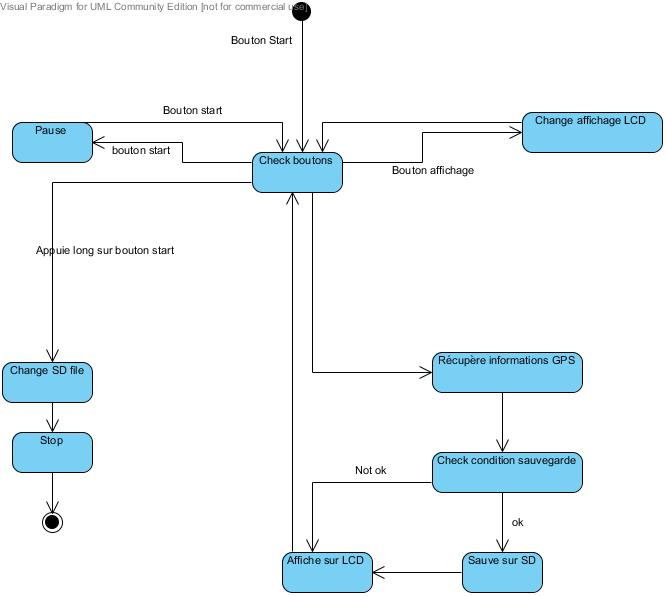
\includegraphics[width=\textwidth]{sequence.jpg}
    \caption{Diagramme de séquence}
    \label{sequence}
\end{figure}

\section{Fonctionnement du programme}

\subsection{Fonctionnement général}

L'affichage sur écran LCD, le système de navigation, la sauvegarde sur carte SD
et la récupération des données du module GPS sont tous gérés par des classes
séparées. La boucle principale ne fait qu'appeler les différents méthodes des
instances de ces classes dans l'ordre. Cette boucle principale gère également
le fonctionnement des boutons, d'une manière proche de celle d'un contrôleur
classique MVC. A chaque passage dans la boucle le système teste si un des
boutons à été appuyé (détection d'évènement) et suivant l'état des boutons, une
méthode adaptée est appelée.

\subsection{Gestion du GPS}

Le module GPS est géré par la classe GPShandler. La fonction principale de
cette classe est \emph{refreshData}. Cette fonction récupère les informations
du modules GPS grâce à une liaison série et la fonction \emph{encode}. Une
boucle permet de récupérer tous les caractères qui arrivent de la liaison série.
La fonction \emph{encode} permet de tester si toute la trame est arrivée, elle
ne renverra vrai que si la trame est lisible. Dans les autres cas la trame
n'est pas complète ou corrompue on continuera à tourner dans la boucle de
réception.

Lorsque toute la trame est arrivée, on met à jour ses attributs privés
\emph{\_lat}, \emph{\_lon}, \emph{\_date}, \emph{\_time} et \emph{\_speed}.
Pour gérer les problèmes de transmission, un \emph{timeout} permet de sortir
de la boucle si la transmission prend trop de temps, afin de ne pas bloquer
l'ensemble du système.

\begin{lstlisting}[caption={resfreshData},label={refreshData}]
// Information refreshing
void GPShandler::refreshData(LCDhandler & lcd) {
unsigned long timer;

if (_isRunning && _nss.available()) {
// Serial Link UP
timer = millis();
do {
    // We try to read a full message, handling transmission timeout in
    // case of communication problems.
    int answer = _nss.read();

    // is the message fully received?
    _isReceived = _gps.encode(answer);

    if (_isReceived) {
        _gps.get_position(&_lat, &_lon, &_fixAge);
        // Time format: hhmmsscc
        // Date format: jjmmaa
        _gps.get_datetime(&_date, &_time, &_fixAge);

        // Converting speed
        _speed = _gps.speed() * KNOT_CONV;

        // Stats : nb chars fed to the gps / nb sentences processed / nb failed checksum tests
        _gps.stats(&_chars, &_sentences, &_failed_checksum);
    }
} while (_nss.available() && !_isReceived && (millis()-timer < TIMEOUT));
    if (millis()-timer > TIMEOUT)
    lcd.notify("Timeout", "ERR");
}
}
\end{lstlisting}

Par ailleurs, on dispose des méthodes permettant de récupérer ces valeurs. La
boucle principale appelle donc à chaque passage \emph{refreshData} et on
utilise les fonctions \emph{get} pour récupérer les dernières valeurs mises à
jour.

\subsection{Gestion du LCD}

Le LCD est géré par la classe \emph{LCDHandler}. Les différentes méthodes
servent à faire de la mise en forme et afficher de manière claire les
informations. Par exemple la fonction \emph{notify} permet d'afficher pendant
quelques secondes une information particulière sur deux lignes. Nous avons
toutefois souhaité que l'affichage ne perturbe à aucun moment le déroulement
des boucles, c'est pourquoi nous n'utilisons pas la procédure \emph{delay}.
Un affichage de plusieurs secondes n'interrompt pas le cycle de rotation de
la boucle principale du programme (loop). Nous comparons plutôt le temps écoulé
avec le délai souhaité à chaque tour de boucle. Ainsi, la réception des trames
GPS peut continuer à s'exécuter.

Les messages longs que nous avons appelés \emph{notifications}permettent
d'afficher un retour en cas d'erreur, d'alerte ou de simple information. Pour
ne pas interrompre l'affichage de ce message malgré le déroulement normal du
programme, nous avons rajouté au système de timer un blocage pour empêcher les
autres fonction d'afficher quoi que ce soit sur l'écran LCD pendant la diffusion
d'une notification.

\begin{lstlisting}[caption={notify}, label={notify}]
void LCDhandler::notify(String s, String type) {
    cls();
    _lcd.print("[" + type + "]");
    _lcd.setCursor(0, 1);
    _lcd.print(s);

    // "A while"
    _isAvailable = false;
    _time = millis();
}

\end{lstlisting}

\subsection{Gestion de la carte SD}

Toute la gestion de la carte SD se trouve dans la classe \emph{SDhandler}.
L'initialisation de la carte se trouve dans la méthode init() de la classe et
non pas dans le constructeur car la SD n'est initiée que dans la méthode setup
de la classe principale du programme, et pas à l'instanciation de la classe
principale

Le système enregistre chaque parcours dans un fichier différent dont le nom est
incrémental (gpslog01.txt, gpslog02.txt, etc).
Pour savoir quel est le fichier à utiliser, notamment lorsque l'on redémarre
le système, un autre fichier contient l'identifiant à utiliser.
Il est créé s'il n'existe pas, et l'identifiant y est écrit/modifié à chaque
incrémentation.

En plus de la méthode d'initialisation, la classe dispose de deux autres
méthodes : \emph{writeCoordinates} et \emph{changeFile}. La première écrit
dans le fichier courant les valeurs passées en paramètres et la deuxième
change de fichier (et met à jour le fichier de numérotation donc).
On appellera cette dernière méthode lorsque l'on stoppe un parcours.

\begin{lstlisting}[caption={changeFile}, label={changeFile}]
/**
*@fn void SDhandler::changeFileName()
*@brief Increment the name of the file and create it
*/
int SDhandler::changeFile() {

    _logFile.close();

    _numFile = _numFile + 1;
    sprintf (_nameFile ,"gpslog%d.txt", _numFile);

    _lastFile = SD.open("lastfile", FILE_WRITE);
    _lastFile.seek(0);
    _lastFile.write(_numFile);
    _lastFile.close();

    _logFile = SD.open(_nameFile, FILE_WRITE);
    if (!_logFile.println ("latitude;longitude;date;time;speed;"))
    return errWrite;
    return 1;

}
\end{lstlisting}

\section{Mode d'emploi}

\begin{figure}[H]
    \centering
    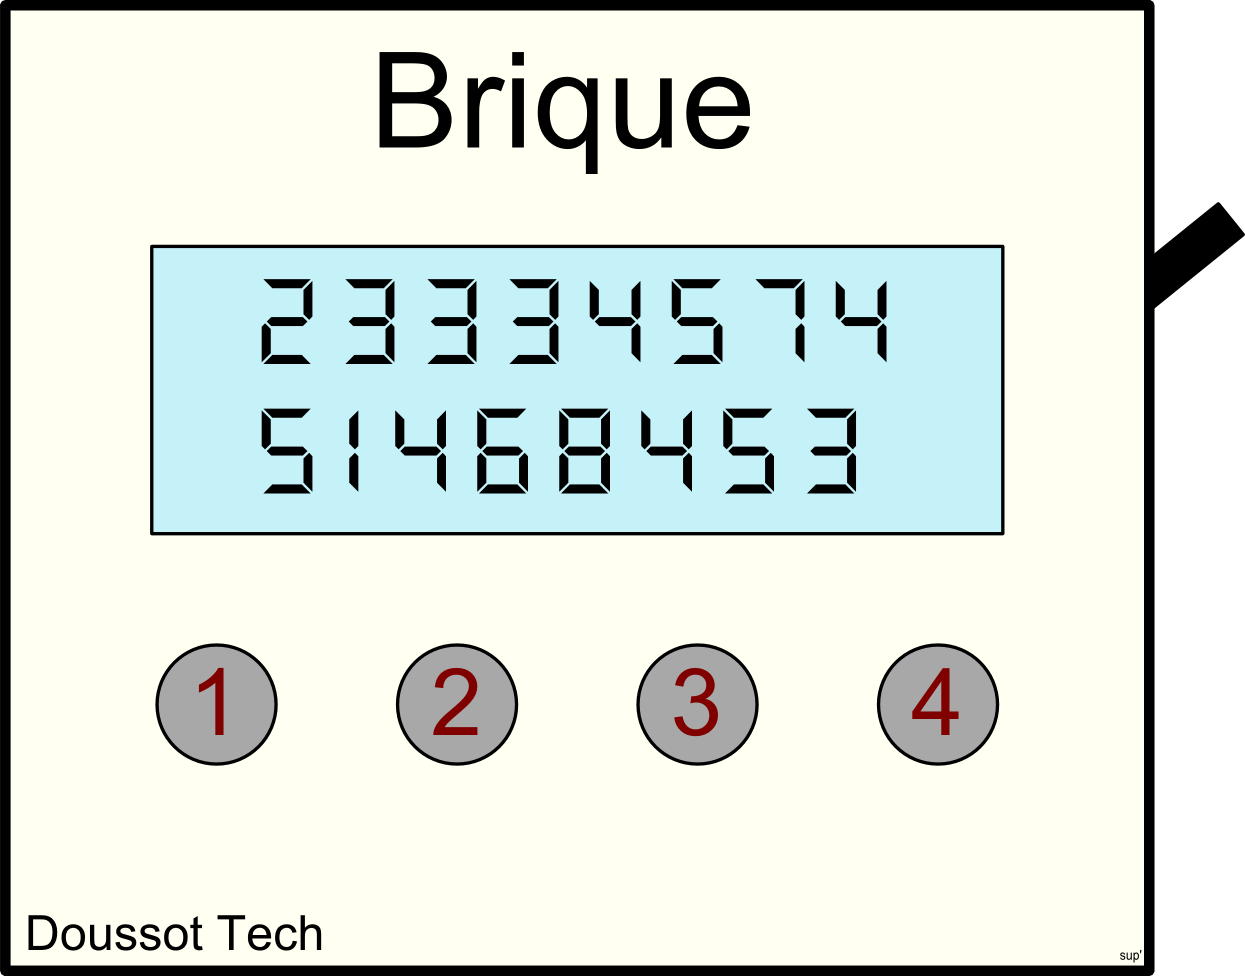
\includegraphics[width=\textwidth]{brique_dessin.png}
    \caption{Schéma de la brique}
    \label{brique_dessin}
\end{figure}

La brique se présente comme un boîtier doté d'un interrupteur sur le côté,
un écran LCD et quatre boutons, qu'on nommera bouton 1, 2, 3 et 4.

\bigskip
L'interrupteur fait passer le circuit sur un fonctionnement par piles, en
l'allumant par la même occasion s'il n'est pas branché.

Une première pression sur le bouton 1 lance la capture de donnée. Une deuxième
pression le met en pause. Appuyer longuement sur le bouton arrête la capture.

Chaque pression sur le bouton 2 fait défiler l'affichage. Dans l'ordre,
l'écran affiche :
\begin{itemize}
    \item la distance parcourue
    \item les coordonnées
    \item la vitesse
    \item diverses informations concernant la réception des trames notamment
\end{itemize}

Le bouton 3 permet de changer le mode de capture. Il y a deux modes, le premier
définit l'enregistrement d'un point sur la carte SD toutes les trois secondes,
le deuxième le fait lorsque la distance entre les deux derniers points est
assez importante. Par défaut le boitier enregistre toutes les trois secondes.

Le bouton 4 ne permet de transférer les fichiers du boitier via le port USB.

\end{document}
